\section{对于MobileNetv3的探索}

\subsection*{概述}

我们推出了新一代的MobileNet网络,该网络基于一种新颖的补充搜索技术的组合。MobileNetV3针对手机CPU进行优化,通过使用硬件感知网络结构搜索(NAS)同时利用NetAdapt算法进行补充,新颖的网络结构发展也对其产生影响。文章首先探索了如何将自动搜索算法与网络设计互补工作从而推进SOTA的高度。通过此研究,我们设计了两个新的MobileNet网络——MobileNetV3-Large与MobileNetV3-Small——这两种网络分别针对于高计算资源环境与低计算资源环境。这两种网络随后被适配与应用于物体检测与语义分割。在语义分割(或者任何密集像素预测)任务中,我们提出了一种新的高效分割解码器LR-ASPP。移动端平台上,我们在分类、检测与分割应用上达到了SOTA。相比于MobileNetV2,MobileNetV3-Large在ImageNet分类中提升了3.2\%的正确率同时减小了20\%延迟;而MobileNetV3-Small在相同延迟的情况下提升了6.6\%的正确率。在COCO数据集上,MobileNetV3-Large在与MobileNetV2正确率相同的情况下可以达到25\%的速度提升。在城市景观分割中,MobileNetV3-Large LR-ASPP在与MobileNetV2 R-ASPP相同正确率的情况下可以有34\%的速度提升。

\begin{figure}[ht]
    \centering
    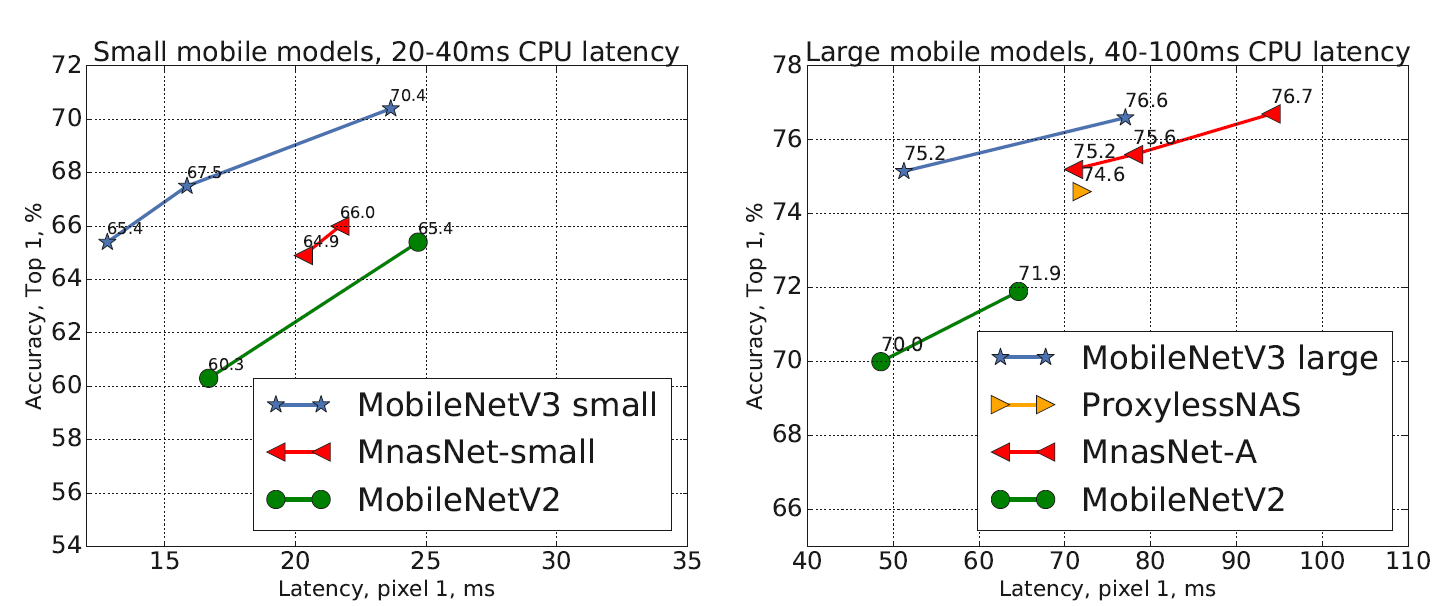
\includegraphics[width=5in]{Figure1.png}
    \caption{在Pixel1手机上的延迟与ImageNet top-1正确率的权衡。所有的模型输入分辨率皆为224.V3 large和V3 small使用0.75,1和1.25的缩放倍数来展示最优边界。所有模型皆利用TFLite框架在单个大核心上运算。MobileNetV3-Small\&Large是我们推出的下一代移动端模型。}
\end{figure}


\begin{figure}[ht]
    \centering
    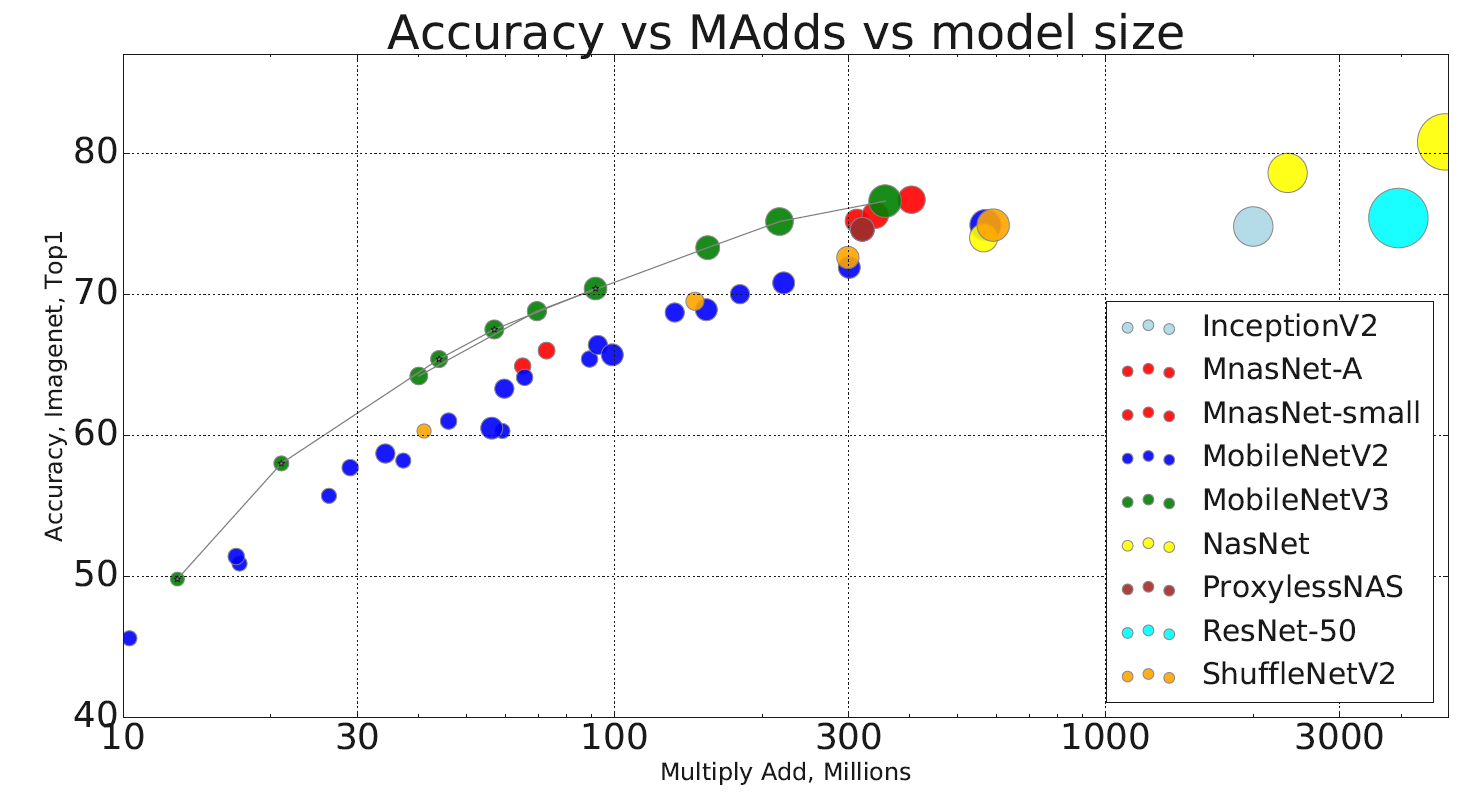
\includegraphics[width=5in]{Figure2.png}
    \caption{Madds和ImageNet top-1正确率的权衡。这个比较允许模型运行在不同的软件框架与硬件平台上。所有的MobileNetV3输入分辨率为224,使用0.35,0.5,0.75,1和1.25的缩放倍率。其他情况可以在第六章节看到。}
\end{figure}


\subsection{介绍}

在移动应用上开始普及的高效神经网络使得移动端的体验有了极大的改变。本地部署使得用户无需将自身隐私上传至服务器就可获得神经网络带来的益处。高效的神经网络不仅通过高正确率与低延迟带给用户体验的提升,同时减少了电能的损耗从而使移动设备获得更好的续航能力。

本文阐述了我们为了提升移动端机器视觉新能而推出的下一代高正确率、高效率神经网络模型,即MobileNetV3-Large与MobileNetV3-Small两种网络模型,的设计过程。这两种模型推动SOTA达到了新的高度,并且展示了如何将自动搜索算法与新的网络结构设计混合工作来设计有效的网络模型。

本文的目的是为了探索一种在移动设备上尽可能平衡正确率与延迟的移动端机器视觉网路模型。为了达到这个目标,我们引入了以下四种技术:

\begin{itemize}
    \item 互补搜索技术
    \item 适用于移动设备的新型高效非线性模型
    \item 新的高效网络设计
    \item 新的高效分割解码器
  \end{itemize}

我们通过实验,证明了以上几种技术在广泛的用途和手机上的价值和有效性。

论文结构如下。我们从第二部分对有关研究的讨论开始。第三部分回顾了适用于移动设备的高效网络模型。第四部分回顾了结构搜索以及MnasNet和NetAdapt算法的互补性。第五部分阐述了新的网络结构设计通过联合搜索提升了模型搜索的效率。第六部分呈献了大量分类、检测与分割的实验数据,展示了模型的有效性与各个模块的功效。第七部分包括总结和今后的工作。

\subsection{相关研究}

近些年,设计一个在正确率与有效性之间平衡的DNN结构已经成为一个热点研究领域。对于推进此领域,手工设计结构与NAS算法都发挥了重要的作用。

SqueezeNet[22]为了压缩参数广泛的使用了1x1卷积核与挤压-扩张模型。近期更多的模型将关注点从减少参数转变到减少计算量(MAdds)以及实际的延迟上。MobileNetV1[19]引入的深度可分离卷积从实质上提升了计算效率。MobileNetV2[39]在此之上引入了一个由翻转残差结构和线性瓶颈的高效资源块。ShuffleNet[49]利用分组卷积与通道乱序进一步减少了MAdds。CondenseNet[21]在训练阶段学习分组卷积以致于维持层间有效连接从而使特征再利用。ShiftNet[46]提出了将移位操作插入点卷积从而减少昂贵的空间卷积。

为了自动化设计网络结构,首先引入强化学习(RL)来寻找具有竞争性正确率的高效网络结构。一个完全可配置的搜索空间将会成指数增长且较难处理。所以结构搜索的前期工作着眼于单元层级的结构搜索。近期,[43]探索了一种结构块层级分层搜索空间,该空间允许在一个网络中存在不同结构块,每个结构块中的分层结构也可不尽相同。为了减少搜索的计算量,在[28,5,45]中使用的可微结构搜索框架进行了梯度优化。而在通过调整现有网络以适应移动平台,[48,15,12]提出了更有效的自动网络简化算法。

通过降低计算精度从而量化网络[23,25,47,41,51,52,37]也是增加网络效率的重要的补充研究方向。最后,知识蒸馏提供了一种从大型网络指导生成小型网络的附加补充方法。

\subsection{高效的移动网络构建块}

移动端模型建立在越来越多的更高效的基础之上。MobileNetV1引入的深度可分离卷积是传统卷积层的有效替代。深度可分离卷积将空间滤波和特征生成机制分离,有效的分解了传统的卷积。深度可分离卷积有两层独立的层组成:较轻量的深度卷积负责空间滤波,计算量较大的1x1点卷积负责特征生成。

MobileNetV2[39]引入了线性瓶颈和翻转的残差结构,目的是利用输入的低层性质使层结构更加有效。这个结构如图~\ref{fig:trans_fig3}所示,由深度可分离卷积,一层1x1扩充卷积和一层1x1的投影卷积组成。瓶颈结构的输入和输出在当通道数相同时将由残差结构相连。该结构在输入和输出的表现形式紧凑的同时,在内部扩充到一个高维度的特征空间,增强了每个通道非线性转换的表达能力。

MnasNet[43]在MobileNetV2的结构之上,在瓶颈块中引入了基于挤压和激励的轻量级注意模型。请注意,此模型中SE插入的位与[20]中基于ResNet中提出的不同。如图~\ref{fig:trans_fig4}所示,该模型将SE置于深度可分离卷积层后的扩增空间中以便应用于最大的表示。

在MobileNetV3中,为了构建出最有效的模型,我们将上述模型组合成构建块。每层的非线性激活函数也升级为改进过的swish。SE结构和swish激活函数中都使用了sigmoid函数,但sigmoid函数很难在定点计算中保持精度,所系我们将其替换为hard sigmoid,此部分我们将在5.2章节讨论。

\begin{figure}[ht]
    \centering
    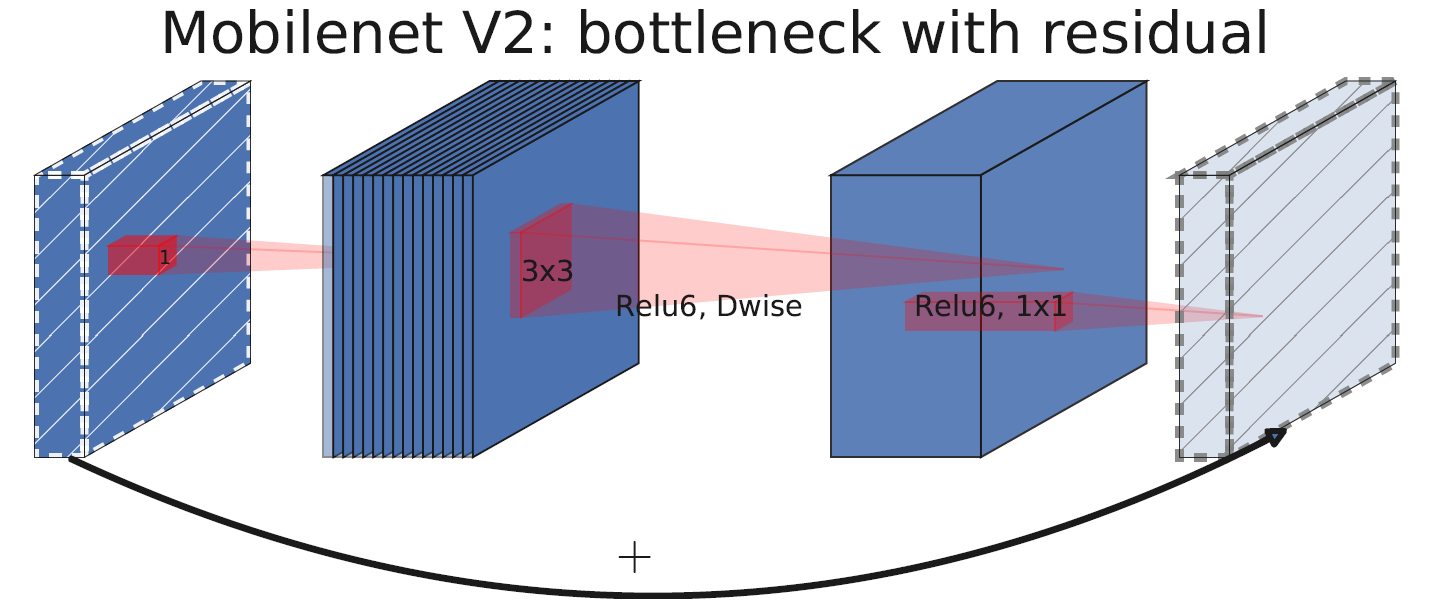
\includegraphics[width=5in]{Figure3.png}
    \caption{MobileNetV2[39]逆残差和线性瓶颈结构块。每个结构块由没有非线性激活函数的较窄的输入层,将输入扩充到较高纬度的空间中扩充层,投影至输出的投影层以及同样没有非线性激活函数的较窄的输出层组成。残差结构连接输入和输出。}
    \label{fig:trans_fig3}
\end{figure}


\begin{figure}[ht]
    \centering
    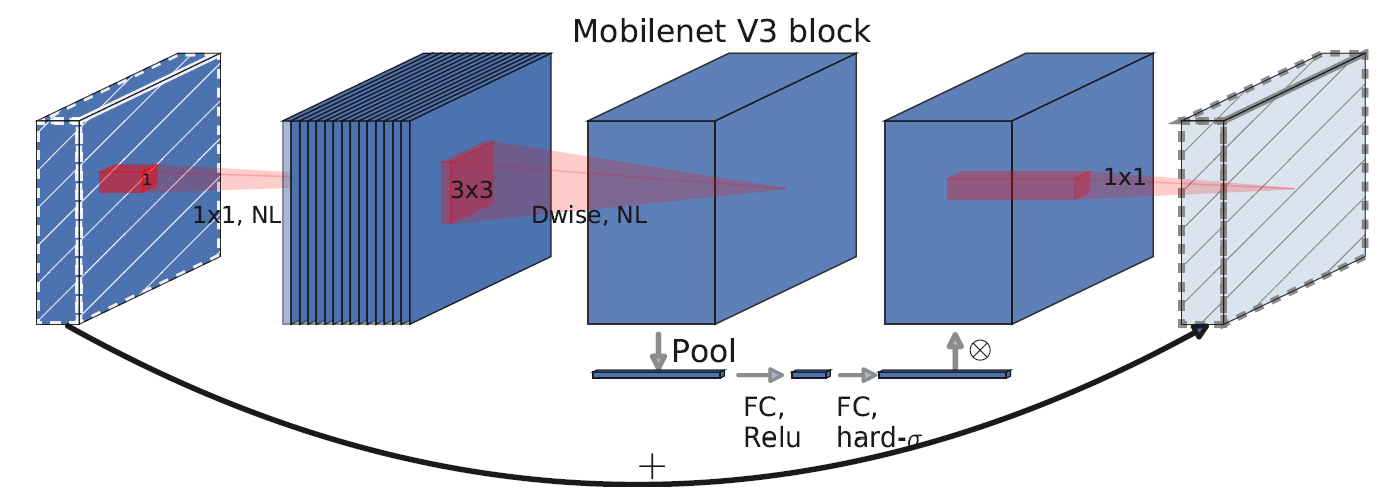
\includegraphics[width=5in]{Figure4.png}
    \caption{MobileNetV2 + SE结构[20]。对比文献[20],我们将SE结构插入残差层。我们在层间使用了不一样的非线性激活函数,具体细节在章节5.2。}
    \label{fig:trans_fig4}
\end{figure}

